\documentclass[a4paper,oneside,UTF8]{article} %A4纸,单面,UTF-8


\newcommand{\kc}{$k$-核}


\usepackage{fancybox,fancyvrb,shortvrb} %也许需要的宏包
\usepackage[heading]{ctex} %用来提供中文支持
\usepackage{amsmath} %
\usepackage{amssymb} %数学符号,定理等环境相关宏包
\usepackage{amsthm}  %
\usepackage{graphicx} %插入图片所需宏包
\usepackage{adjustbox}  %也许需要的宏包
\usepackage{xspace} %提供一些好用的空格命令
\usepackage{tikz-cd} %画交换图需要的宏包
\usepackage{url} %更好的超链接显示
\usepackage{array} %表格相关的宏包
\usepackage{booktabs} %表格相关的宏包
\usepackage{caption} %实现图片的多行说明
\usepackage{float} %图片与表格的更好排版
\usepackage{fontspec}
\usepackage{xeCJK}
\usepackage{subfigure}
\usepackage{multirow}
\usepackage{weiwAlgorithm}
\usepackage{algorithmicx}
\usepackage{lineno,hyperref}
\usepackage{comment}
\usepackage{ulem} %for sout

\usepackage{ulem} %更好的下划线

\usepackage[ top=2.5cm, bottom=2.0cm, left=3.0cm, right=2.0cm]{geometry} %设置页边距

%\usepackage{fontspec}                   %设置字体需要的宏包
\setmainfont{Times New Roman}           %设置西文字体为Times New Roman
\setCJKmainfont{simsun.ttc}                 %设置中文字体为宋体
%\setCJKmainfont[BoldFont=SimHei]{SimSun}
%\setCJKmonofont{SimSun}    % 设置缺省中文字体              %设置中文字体为宋体

\renewcommand{\normalsize}{\zihao{-4}}  %设置正文字号为小四

\linespread{1.5} %1.5倍行距

\showboxdepth=5
\showboxbreadth=5 

\setcounter{secnumdepth}{5}                                                                                     %
\ctexset { section = { name={,、},number={\chinese{section}},format={ \heiti \zihao {-4}} } }         %
\ctexset { subsection = { name={(,)},number={\chinese{subsection}},format={ \heiti \zihao {-4}} } } %设置各级系统的编号格式
\ctexset { subsubsection = { name={,.},number={\arabic{subsubsection}},format={\heiti \zihao {-4}} } }          %
\ctexset { paragraph = { name={(,)},number={\arabic{paragraph}},format={\heiti \zihao {-4}} } }               %
\ctexset { subparagraph = { name={,)},number={\arabic{subparagraph}},format={\heiti \zihao {-4}} } }           %

\usepackage[bottom,perpage]{footmisc}               %脚注,显示在每页底部,编号按页重置
\renewcommand*{\footnotelayout}{\zihao{-5}\songti}  %设置脚注为小五号宋体
\renewcommand{\thefootnote}{[\arabic{footnote}]}    %设置脚注标记为  [编号]
                      %脚注的反向超链接


\usepackage{fancyhdr}               %
\renewcommand{\headrulewidth}{0pt}  %
\lhead{}                            %
\chead{}                            %将页眉页脚设置为:仅在右下角显示页码
\rhead{}                            %
\lfoot{}                            %
\cfoot{\thepage}                            %
\rfoot{}                    %

\usepackage{xcolor} %彩色的文字

%\usepackage[hidelinks]{hyperref} %各种超链接必备

\usepackage{endnotes}                                                           %
\renewcommand{\enotesize}{\zihao{-5}}                                           %
\renewcommand{\notesname}{\heiti \zihao {-4} 尾注}                              %
\renewcommand\enoteformat{                                                      %
  \raggedright                                                                  %尾注的相关设置
  \leftskip=1.8em                                                               %
  \makebox[0pt][r]{\theenmark. \rule{0pt}{\dimexpr\ht\strutbox+\baselineskip}}  %
}                                                                               %
\renewcommand\makeenmark{\textsuperscript{[尾注\theenmark]}}                    %
\usepackage{footnotebackref}  


\newtheorem{theorem}{\heiti 定理}[section]      %
\newtheorem*{theorem*}{\heiti 定理}             %
\newtheorem{lemma}[theorem]{\heiti 引理}        %
\newtheorem*{lemma*}{\heiti 引理}               %
\newtheorem{corollary}[theorem]{\heiti 推论}    %
\newtheorem*{corollary*}{\heiti 推论}           %
\newtheorem{definition}[theorem]{\heiti 定义}   %
\newtheorem*{definition*}{\heiti 定义}          %
\newtheorem{conjecture}[theorem]{\heiti 猜想}   %将各种常用环境设置为中文
\newtheorem*{conjecture*}{\heiti 猜想}          %
\newtheorem{problem}[theorem]{\heiti 问题}      %
\newtheorem*{problem*}{\heiti 问题}             %
\newenvironment{solution}                       %
  {\renewcommand\qedsymbol{$\blacksquare$}      %
  \begin{proof}[\heiti \bf 解]}                 %
  {\end{proof}}                                 %
\renewcommand*{\proofname}{\heiti \bf 证明}     %

\allowdisplaybreaks %允许公式跨页显示




\usepackage[bibstyle=gb7714-2015,citestyle=gb7714-2015,hyperref=true,backend=biber,sorting=none,gbpub=false]{biblatex}
%\usepackage[bibstyle=gb7714-2015,citestyle=gb7714-2015,hyperref=true,backend=biber,sorting=none]{biblatex} %使用biblatex管理文献,输出格式使用gb7714-2015标准,后端为biber

\usepackage{titletoc}
\titlecontents{section}[0pt]{\addvspace{2pt}\filright}
{\contentspush{\thecontentslabel\ }}
{}{\titlerule*[8pt]{.}\contentspage}

\usepackage[titletoc,title]{appendix} %提供了附录支持并显示在目录中
\renewcommand{\appendixtocname}{附录} %

\newcommand{\apdx}[1] { %
\clearpage              %重定义生成附录的命令,使得每个附录都单独成页
\section{#1}}           %


 %加载各宏包以及本模板的主要设置
\addbibresource{ref.bib} %加载bib文件(参考文献)

\begin{document}
\pagestyle{empty} %不对正文前的各页面使用页眉页脚

\thispagestyle{empty}
\begin{titlepage}
    \newcommand{\TitleCHS}{} %中文标题

\newcommand{\TitleENG}{} %英文标题

\newcommand{\Author}{} %作者名字

\newcommand{\StudentID}{} %学号

\newcommand{\Department}{软件工程学院} %学院

\newcommand{\Major}{软件工程} %专业


\newcommand{\Supervisor}{} %导师名字

\newcommand{\SupervisorTitle}{教授} %导师职称

\newcommand{\CompleteYear}{2022} %毕业年份

\newcommand{\CompleteMonth}{6} %毕业月份

\newcommand{\KeywordsCHS}{} %中文关键词

\newcommand{\KeywordsENG}{} %英文关键词

    \setlength\parindent{0pt} 
\parbox[t][2cm][t]{\textwidth}{\textbf{\Large{\CompleteYear 届本科生学士学位论文}}  \hfill \Large{学校代码:~\underline{10269}}} 

\parbox[t][10.0cm][t]{\textwidth}{
    \begin{center}

\includegraphics[height=9.5cm]{figures/ECNUlogo.png}
    \end{center} }

\parbox[t][2.5cm][t]{\textwidth   }{\Huge
\begin{center} {\bf  \TitleCHS } \end{center} } 

\parbox[t][4.5cm][t]{\textwidth}{\huge
\begin{center} {\bf  \TitleENG } \end{center} }

\parbox[t][6cm][c]{\textwidth}{ {\Large
\begin{center}
    \renewcommand{\arraystretch}{1.0}
    \begin{tabular}{p{0cm}p{5em}l@{\extracolsep{1em}}l}
    ~ & 姓\hfill 名:& & \underline{{\bf\makebox[4.5cm][c]{\Author}}}\\
    ~ & 学\hfill 号: & & \underline{{\bf\makebox[4.5cm][c]{\StudentID}}} \\
    ~ & 学\hfill 院: & & \underline{{\bf\makebox[4.5cm][c]{\Department}}} \\
    ~ & 专\hfill 业: & & \underline{{\bf\makebox[4.5cm][c]{\Major}}} \\
    ~ & 指\hfill 导\hfill 教\hfill 师:    & & \underline{{\bf\makebox[4.5cm][c]{\Supervisor}}}\\
    ~ & 职\hfill 称: & & \underline{{\bf\makebox[4.5cm][c]{\SupervisorTitle}}} \\
    \multicolumn{4}{c}{\bf{\CompleteYear 年 \CompleteMonth 月}}
    \end{tabular}
    \end{center} }  }
\end{titlepage}  %插入内封面
\clearpage                                          %       
\thispagestyle{empty}                               %

\vspace{10mm}
\begin{center}
{\Large\bf\heiti\zihao{-4} 华东师范大学学位论文诚信承诺}   %
\end{center}

%%%%%%%%%%%%%%%%%%%%%%%%%%%%%%%%%%%%%%%%%%%%%%%%%%%%%


本毕业论文是本人在导师指导下独立完成的,内容真实、可靠。本人在撰写毕业论文过程中不存在请人代写、抄袭或者剽窃他人作品、伪造或者篡改数据以及其他学位论文作假行为。

本人清楚知道学位论文作假行为将会导致行为人受到不授予/撤销学位、开除学籍等处理(处分)决定。本人如果被查证在撰写本毕业论文过程中存在学位论文作假行为,愿意接受学校依法作出的处理(处分)决定。

\vspace{5mm}
承诺人签名: \hfill { 日期:2022年\quad 月\quad 日}


\vspace{30mm}
\begin{center}
{\Large\bf\heiti\zihao{-4} 华东师范大学学位论文使用授权说明}   %
\end{center}

本论文的研究成果归华东师范大学所有,本论文的研究内容不得以其它单位的名义发表。本学位论文作者和指导教师完全了解华东师范大学有关保留、使用学位论文的规定,即:学校有权保留并向国家有关部门或机构送交论文的复印件和电子版,允许论文被查阅和借阅;本人授权华东师范大学可以将论文的全部或部分内容编入有关数据库进行检索、交流,可以采用影印、缩印或其他复制手段保存论文和汇编本学位论文。

保密的毕业论文(设计)在解密后应遵守此规定。

\vspace{5mm}
作者签名:\qquad\qquad\qquad\qquad\quad             导师签名:          \hfill { 日期:2022年\quad 月\quad 日}


\newpage %插入签名页面

\tableofcontents %生成目录

\clearpage
\pagestyle{fancy} %开始使用页眉页脚

\pagenumbering{Roman}
\setcounter{page}{1}

% 除了中英文摘要,通常不需要修改其他内容

\clearpage
%\thispagestyle{empty}
\newcommand{\TitleCHS}{} %中文标题

\newcommand{\TitleENG}{} %英文标题

\newcommand{\Author}{} %作者名字

\newcommand{\StudentID}{} %学号

\newcommand{\Department}{软件工程学院} %学院

\newcommand{\Major}{软件工程} %专业


\newcommand{\Supervisor}{} %导师名字

\newcommand{\SupervisorTitle}{教授} %导师职称

\newcommand{\CompleteYear}{2022} %毕业年份

\newcommand{\CompleteMonth}{6} %毕业月份

\newcommand{\KeywordsCHS}{} %中文关键词

\newcommand{\KeywordsENG}{} %英文关键词

\centerline{\bf \heiti \zihao{-3}\TitleCHS}
\phantomsection
\addcontentsline{toc}{section}{摘要}
\renewcommand\abstractname{\heiti\zihao{-4} 摘要}
\begin{abstract}\zihao{5}\songti
    { % 中文摘要
        网络的结构稳定性反映了网络维持其可持续服务的能力。
    }
    \newline
    \newline
    {\bf \heiti\zihao{5} 关键词:} \zihao{5}{\songti \KeywordsCHS}
\end{abstract}

\clearpage
\centerline{\bf \heiti \zihao{-3}\TitleENG}
\renewcommand\abstractname{\zihao{-4} Abstract}
\phantomsection
\addcontentsline{toc}{section}{Abstract}
\begin{abstract}\zihao{5}
    { % 英文摘要
        The structural stability of a network reflects the ability of the network to maintain a sustainable service.
    }
    \newline
    \newline
    {\bf \zihao{5} Keywords: } {\zihao{5} \KeywordsENG}
\end{abstract}
 %生成中英文摘要及关键词


\clearpage
\pagenumbering{arabic}
\setcounter{page}{1} %论文页码从正文开始记数

\section{简介}

网络用户逐渐流失,最终瓦解了~\cite{friendster,DBLP:conf/cosn/GarciaMS13}。

\begin{figure}
	\centering
	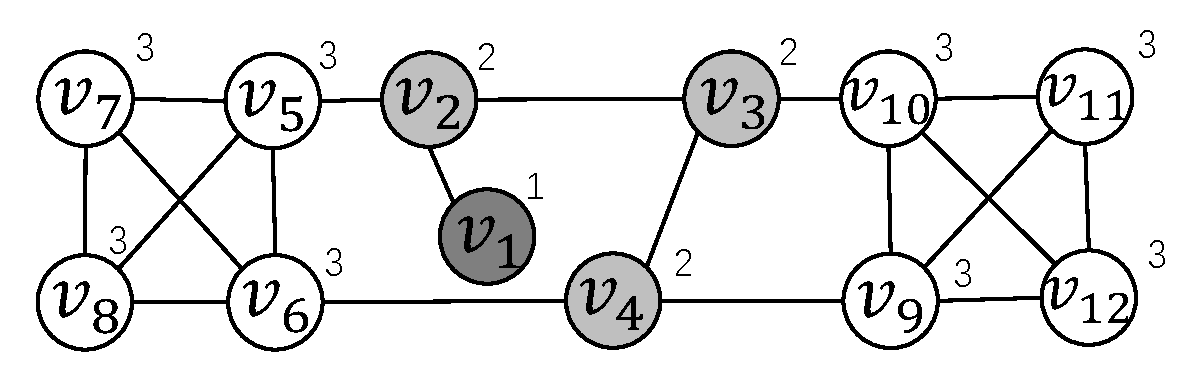
\includegraphics[width=0.7\linewidth]{figures/toy-example.pdf}
    %\vspace{-2mm}
	\caption{A Toy Graph (The coreness of each vertex is marked near the vertex)}%
	\label{fig:example}
\end{figure}

\begin{table}[t]
	\centering%
	\caption{Collapsed $k$-Core v.s. Collapsed Coreness in Figure~\ref{fig:example}}
	\label{tab:example}
	%\renewcommand{\arraystretch}{1.3}%
	%\resizebox{0.48\textwidth}{!}{
	\begin{tabular}{|l|c|c|c|c|}
	\hline
		\bf{Problem} &  \bf{Input} & \bf{Collapser} & \bf{Followers} & \bf{Coreness} \\
		\hline
		\hline
\multirow{2}{*}{Collapsed $k$-Core} & $k=2,b=1$ & $v_3$ & $v_2$ & from $2$ to $1$ \\

\cline{2-5} & $k=3,b=1$ & $v_6$ & $v_{5},v_{7},v_{8}$ & from $3$ to $2$ \\
\hline
\multirow{2}{*}{Collapsed Coreness} & \multirow{2}{*}{$b=1$} & \multirow{2}{*}{$v_5$} & $v_2$ & from $2$ to $1$ \\
\cline{4-5} & & & $v_6,v_7,v_8$ & from $3$ to $2$ \\

		\hline
	\end{tabular}
	%}
\end{table}

\section{问题定义}

\begin{algorithm}[t]
    \SetVline % save space
    \SetFuncSty{textsf}
    \SetArgSty{textsf}
	\caption{CoreDecomp($G,D$)}
	\label{algo:cd}
	\Input{a graph $G$, a set $D$ of collapsed vertices}
	\Output{$c^D(u,G)$ for each $u\in V(G) \setminus D$}
    	\ForEach{$u\in D$}
    	{
    	    \ForEach{$v\in N(u,G)$}
    	    {
    	        \State{$d(v)\leftarrow d(v)-1$}
    	    }
    	    \State{remove $u$ and its incident edges from $G$}
    	}
    	\State{$k\leftarrow 1$}
    	\While{exist vertices in $V(G)  \setminus D$}
    	{
    	    \While{$\exists u\in V(G)  \setminus D$ with $d(u) < k$}
    	    {
    	        \ForEach{$v\in N(u,G)$}
    	        {
    	            \State{$d(v)\leftarrow d(v)-1$}
    	        }
    	        \State{remove $u$ and its incident edges from $G$}
    	        \State{$c^D(u,G)\leftarrow k-1$}
    	    }
    	    \State{$k\leftarrow k+1$}
    	}
    	\Return{$c^D(u,G)$ for each $u\in V(G)  \setminus D$}
\end{algorithm}

\cleardoublepage                                      %
\phantomsection                                       %生成参考文献
\addcontentsline{toc}{section}{参考文献}               %
\printbibliography[title={\centering \heiti \zihao {-3}参考文献}] %

\clearpage                                       %



% \begin{appendices}                               %
% \renewcommand{\thesection}{\chinese{section}}  %生成附录
% \input{./ending/Appendix.tex}                    %
% \end{appendices}                                 %

% \clearpage                           %生成感谢
% \input{./ending/acknowledgement.tex} %

\end{document}